\documentclass{article}
\usepackage[utf8]{inputenc}
\usepackage{graphicx}

\title{IE 498 HW3}
\author{Yifan Shi(yifans16)}
\date{March 7, 2020}

\begin{document}

\maketitle


First of all, I set the learning rate to be 0.0005, batch size 
to be 40 and number of epochs to be 10. I totally set 8 
convolution layers, 2 max-pooling layers and 2 fully connected 
layers. I also use batch normalization and dropout both for 5 
times throughout my network. I performe the data augmentation 
right after the permutiation. I only use random horizontal and 
vertical flip with probability of 0.1 because I am not able to 
figure out how to adjust the brightness, contrast and color 
saturation on the normalized data. 


The input layer is 3*32*32. The $1^{st}$ and $2^{nd}$ convolution 
layers have kernels in size of 3*3 with 32 channels and the padding 
size is 2. I also do the batch normalization on the former layer. 
The output is now 32*32*32 and after the 2*2 max-pooling layer, 
the output is 32*16*16. 


After applying the dropout with rate of 0.2, the $3^{rd}$ 
and $4^{th}$ convolution layers have kernels in size of 3*3 with 
64 channels and the padding size is 2. I also do the batch 
normalization on the former layer. The output is now 64*16*16 
and after the 2*2 max-pooling layer, the output is 64*8*8. 


After applying the dropout with rate of 0.25, the $5^{th}$ and $6^{th}$ 
convolution layers have kernels in size of 3*3 with 64 channels 
and the former one of them has padding size of 2. I also do the batch 
normalization on the former layer. The output is now 64*6*6.


After applying the dropout with rate of 0.25, the $7^{th}$ and $8^{th}$ 
convolution layers have kernels in size of 3*3 with 128 channels 
and the former one of them has padding size of 2. I also do the batch 
normalization on both of the layers. The output is now 128*4*4.


After applying the dropout with rate of 0.3, the $1^{st}$ fully 
connected layer has weight in size of 2048*500 and the output is 
1*500. Then the dropout rate is 0.5, and the $2^{nd}$ fully connected 
layer has weight in size of 500*10 which makes the very last output 
layer to be 1*10.


The Testing accuracy is 83 percent which is shown below. I also 
print out the running time and loss for each epoch. 


\newpage

\begin{figure}[h]
    \centering
    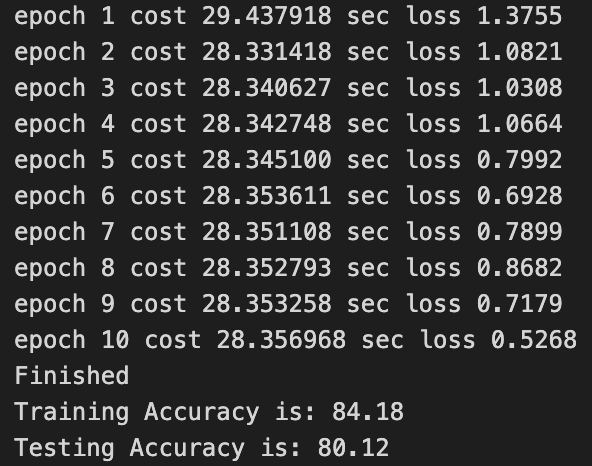
\includegraphics[scale=0.6]{accuracy.png}
  \end{figure}
\centering Figure\ 1: Epoch Loss and Accuracy.


\end{document}